% Sección (v) Resultados y discusión. Se inserta en main.tex después de la
% Configuración experimental:
%   \clearpage
%   % Sección (v) Resultados y discusión. Se inserta en main.tex después de la
% Configuración experimental:
%   \clearpage
%   % Sección (v) Resultados y discusión. Se inserta en main.tex después de la
% Configuración experimental:
%   \clearpage
%   % Sección (v) Resultados y discusión. Se inserta en main.tex después de la
% Configuración experimental:
%   \clearpage
%   \input{resultados}
% Cada cifra lleva su fuente en un comentario «% fuente: ruta».
% R = experiments/results. Las tablas y las figuras se generan con scripts.
% D = R/entrega3_revision/descriptivos.csv (descriptivo, no prerregistrado).
\section{Resultados y discusión}
\label{sec:resultados}\label{res-ini}
% Evita líneas viudas y huérfanas en esta sección y en la conclusión.
% \@clubpenalty es el valor que LaTeX restaura después de cada título.
\makeatletter\@clubpenalty=10000\makeatother
\clubpenalty=10000\widowpenalty=10000

\subsection{Tabu aporta la mayor parte de la mejora}
\label{subsec:absolutos}
El estudio completó los 960 pares sin fallos y su auditoría recalculó los 5.760
calendarios, todos factibles.
% fuente: R/entrega2_congestion_90_109/verification.json
El 51,8~\% de las soluciones de Tabu uniforme y D-MAB terminó con espera, entre
45,0~\% y 57,5~\% según el tamaño.
% fuente: R/entrega2_exploratorio/espera_por_tamano.csv
La Tabla~\ref{tab:descriptiva} muestra que Tabu uniforme ya mejora en 11,2~\% a la
mejor regla constructiva. UCB1 llega a 12,0~\%: cambiar la selección agrega menos de un
punto.
% fuente: D (improvement_over_best_rule)

\begin{table}[!ht]
 \centering
 \caption{Resultados en congestión (48 instancias, semillas 90--109; menor es mejor). RPD: respecto del mejor valor conocido, no del óptimo. Negrita: menor valor de cada bloque.}
 \label{tab:descriptiva}
 \scriptsize\setlength{\tabcolsep}{4pt}
 \input{tablas/tabla_descriptiva}
\end{table}

\subsection{La evidencia sobre D-MAB frente a Tabu uniforme no es concluyente}
\label{subsec:c1}
En C1 (Tabla~\ref{tab:comparaciones}), la diferencia media fue $-0{,}793$, con
IC~95~\% [$-1{,}850$; $+0{,}279$] y $p$ de Holm 0,041.
% fuente: R/entrega2_congestion_90_109/comparisons.csv (C1)
Wilcoxon rechaza la igualdad, pero el intervalo incluye el cero. Por tanto, la regla
prerregistrada no respalda la hipótesis primaria. El desacuerdo se relaciona con el
bootstrap: su error estándar es 1,62 veces el de las medias por instancia.
% fuente: D (bootstrap_se_ratio, C1)
Aunque es conservador, se fijó antes y no lo cambiamos.

El intervalo incluye beneficios y perjuicios mayores que el umbral de 0,25. Además,
la DE de las diferencias fue 13,21 y no la supuesta de 7,03. Así, la potencia para
detectar 0,65 cayó a 0,32, y el resultado no prueba equivalencia.
% fuente: R/entrega2_exploratorio/potencia_realizada.csv
La espera total bajó con D-MAB de 9,31 a 8,29 minutos. El \emph{makespan}, en
cambio, subió levemente, de 287,56 a 287,79.
% fuente: R/entrega2_congestion_90_109/descriptive.csv

\begin{table}[!ht]
 \centering
 \caption{Diferencias de $f$, en unidades del objetivo (semillas 90--109, 960 pares); negativo favorece a la alternativa. Negrita: cumple los tres criterios de la regla, que solo era vinculante para C1. Las columnas por tamaño son descriptivas, con 12 instancias cada una.}
 \label{tab:comparaciones}
 \scriptsize\setlength{\tabcolsep}{4pt}
 \input{tablas/tabla_comparaciones}
\end{table}

\subsection{La cartera gana al prolongado, pero no a repetir la búsqueda}
\label{subsec:cartera}
La cartera superó al Tabu prolongado (C2), pero no se distinguió de dos Tabu
independientes (C3). Por tanto, no atribuimos su ganancia al aprendizaje. La
explicación más simple es el estancamiento. En 546 de las 960 corridas (56,9~\%),
el Tabu prolongado no mejoró después de la evaluación 3.030.
% fuente: R/entrega3_descriptivos/descriptivos.csv
La ventaja aparece con 25 y 30 cirugías; con 15 y 20, la cartera es peor en media.
Además, el error tipo~I simulado de C2 fue 0,082.
% fuente: R/entrega2_potencia/simulacion.csv

\subsection{UCB1 supera a D-MAB y a Tabu uniforme, según el tamaño}
\label{subsec:reinicio}
En C4, quitar el reinicio mejoró el resultado: con 25 cirugías, UCB1 venció a D-MAB
en las 12 instancias.
% fuente: D (instances_better_25, C4)
Con 15, en cambio, D-MAB fue mejor en media. El contraste exploratorio entre UCB1
y Tabu uniforme había dado $-2{,}617$.
% fuente: R/entrega2_exploratorio/contrastes.csv
Por eso, lo confirmamos con un protocolo propio y semillas nuevas. En E1, la
diferencia fue $-2{,}749$, con IC [$-4{,}069$; $-1{,}453$] y $p$ menor que 0,001
(Figura~\ref{fig:forest}).
% fuente: R/entrega3_confirmacion_ucb1/comparisons.csv (E1)

E1 cumple la regla y mejora en 38 de 48 instancias, pero equivale a solo 0,92~\%
de $f$. Además, depende del tamaño. Con 15, 20, 25 y 30 cirugías dio $+0{,}12$,
$-2{,}96$, $-3{,}91$ y $-4{,}25$: con 15 no hay ventaja.
% fuente: D (instances_better, relative_difference y difference_<tamaño>, E1)

\begin{figure}[!ht]
 \centering
 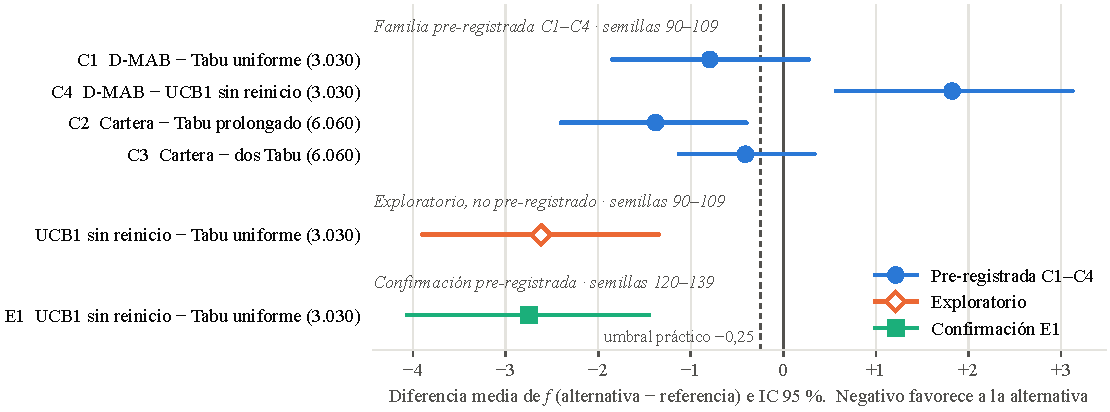
\includegraphics{figuras/forest_comparaciones}
 \caption{Diferencia media de $f$ e IC~95~\%; negativo favorece a la alternativa. Cada grupo es un análisis distinto.}
 \label{fig:forest}
\end{figure}

\subsection{La mejora de UCB1 cuesta cómputo y dispersión}
\label{subsec:costo}
Igual número de evaluaciones no significa igual cómputo. UCB1 repite más candidatos:
decodificó 10,1~\% más propuestas que Tabu uniforme y tardó 10,2~\% más (9,8~\%
en E1). D-MAB tardó 4,0~\% más.
% fuente: D (decoded_overhead, time_overhead)
UCB1 también fue más variable entre semillas, con DE de 9,36 frente a 8,72. En E1
se repitió el patrón: 9,89 frente a 8,90.
% fuente: D (sd)
La Figura~\ref{fig:distribucion} muestra que las distribuciones se superponen y que
la ventaja media de UCB1 se mantiene hasta el final.

En el piloto a igual tiempo, D-MAB fue peor que Tabu uniforme en tres de los cuatro
tamaños: $+0{,}21$, $-2{,}30$, $+2{,}70$ y $+6{,}00$. Son solo cinco semillas
por tamaño y el piloto no incluyó UCB1.
% fuente: R/entrega2_tiempo_110_114/summary.csv

\begin{figure}[!ht]
 \centering
 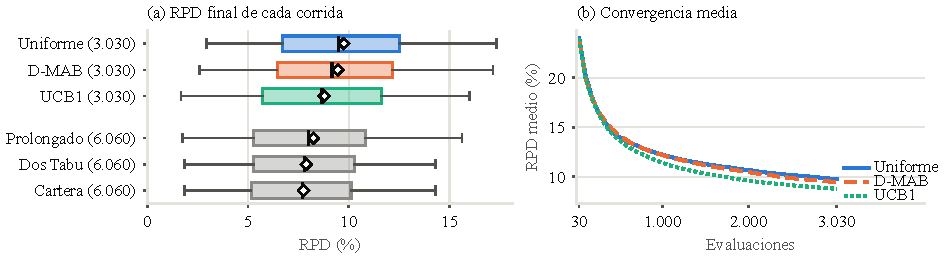
\includegraphics{figuras/distribucion_convergencia}
 \caption{Semillas 90--109. (a) RPD de 960 corridas por método: caja intercuartil, mediana, media (rombo) y percentiles 5--95. (b) RPD medio del mejor valor durante la búsqueda.}
 \label{fig:distribucion}
\end{figure}

\subsection{En el catálogo estándar los efectos no fueron consistentes}
\label{subsec:estandar}
Con la configuración vigente (semillas 40--59), los signos se invirtieron respecto
de la congestión. UCB1
menos uniforme dio $+1{,}182$; D-MAB menos uniforme, $+0{,}577$; y D-MAB menos
UCB1, $-0{,}605$.
% fuente: D (40-59)
Con la configuración anterior (semillas 20--39, $c=1$, $\lambda=0{,}35$), esas diferencias fueron
$-0{,}455$, $-0{,}513$ y $-0{,}058$.
% fuente: D (20-39)
En las semillas 60--79, D-MAB dio $+0{,}108$ frente a uniforme. La cartera dio
$-0{,}656$ frente al prolongado y $+0{,}134$ frente a dos Tabu.
% fuente: D (60-79)
Son descriptivos, con 12 instancias, y ninguno sustenta una superioridad.

\subsection{Discusión: bajo congestión ayuda UCB1, no el reinicio}
\label{subsec:discusion}
Los resultados responden la pregunta solo bajo escasez de cirujanos e igual número
de evaluaciones. Allí no identificamos una mejora concluyente de
D-MAB, mientras que UCB1 sí mejora, sobre todo desde 20 cirugías. La evidencia
señala al reinicio, con la configuración probada, como perjudicial en ese catálogo.
No demuestra que toda detección de cambios lo sea.

Una explicación plausible es que el detector confunde el agotamiento normal de la
búsqueda con un cambio entre operadores. Page--Hinkley detecta caídas de recompensa,
y las mejoras escasean al estancarse la búsqueda. D-MAB reinició una mediana de 24
veces por corrida, y cada reinicio borra sus estimaciones.
% fuente: R/entrega3_descriptivos/descriptivos.csv
La reparación no basta para explicarlo, porque afecta a todos. Alteró 46,6~\% de los
candidatos en uniforme, 44,0~\% en D-MAB y 40,1~\% en UCB1.
% fuente: R/entrega3_descriptivos/descriptivos.csv
Como no medimos si cambia el mejor operador, el mecanismo sigue siendo una hipótesis.

Este hallazgo concuerda con una parte de \textcite{dacosta2008}. En su escenario de
recompensas binarias, de alta varianza, el bandido sin reinicio superó a D-MAB.
Nuestra señal también es irregular: en el diagnóstico estándar, solo 3,9~\% de las
propuestas recibió recompensa positiva.
% fuente: R/entrega2_diagnostico_115_119/summary.csv
\textcite{dolatkhah2026} reinician con otra regla, una brecha entre operadores, por
lo que su resultado no valida este detector. \textcite{yin2026} miden brechas
frente a cotas; nuestro RPD, en cambio, no mide la distancia al óptimo.

E1 tampoco prueba que aprender sea la causa. UCB1 dedicó 39,1~\% de sus evaluaciones
al cambio de sala de anestesia, frente a 19,6~\% del uniforme.
% fuente: D (share_room_1)
Una mezcla fija con ese sesgo podría igualarlo. Además, confirmar con semillas
nuevas sobre las mismas instancias no mide generalización. Tampoco evaluamos
una cartera con UCB1.%
\label{res-fin}

% Cada cifra lleva su fuente en un comentario «% fuente: ruta».
% R = experiments/results. Las tablas y las figuras se generan con scripts.
% D = R/entrega3_revision/descriptivos.csv (descriptivo, no prerregistrado).
\section{Resultados y discusión}
\label{sec:resultados}\label{res-ini}
% Evita líneas viudas y huérfanas en esta sección y en la conclusión.
% \@clubpenalty es el valor que LaTeX restaura después de cada título.
\makeatletter\@clubpenalty=10000\makeatother
\clubpenalty=10000\widowpenalty=10000

\subsection{Tabu aporta la mayor parte de la mejora}
\label{subsec:absolutos}
El estudio completó los 960 pares sin fallos y su auditoría recalculó los 5.760
calendarios, todos factibles.
% fuente: R/entrega2_congestion_90_109/verification.json
El 51,8~\% de las soluciones de Tabu uniforme y D-MAB terminó con espera, entre
45,0~\% y 57,5~\% según el tamaño.
% fuente: R/entrega2_exploratorio/espera_por_tamano.csv
La Tabla~\ref{tab:descriptiva} muestra que Tabu uniforme ya mejora en 11,2~\% a la
mejor regla constructiva. UCB1 llega a 12,0~\%: cambiar la selección agrega menos de un
punto.
% fuente: D (improvement_over_best_rule)

\begin{table}[!ht]
 \centering
 \caption{Resultados en congestión (48 instancias, semillas 90--109; menor es mejor). RPD: respecto del mejor valor conocido, no del óptimo. Negrita: menor valor de cada bloque.}
 \label{tab:descriptiva}
 \scriptsize\setlength{\tabcolsep}{4pt}
 % Generado por experiments/scripts/tabla_descriptiva.py. No editar a mano.
% fuente: experiments/results/entrega3_revision/descriptivos.csv
\begin{tabular}{@{}lrrrrrrrrr@{}}
 \toprule
 & \multicolumn{5}{c}{Objetivo $f$ (unidades)} & \multicolumn{3}{c}{Componentes (min)} & \\
 \cmidrule(lr){2-6}\cmidrule(lr){7-9}
 Método & Mejor & Media & Peor & DE & RPD (\%) & $C_{\max}$ & $\sum W$ & $\max W$ & $t$ (s)\\
 \midrule
 FIFO & -- & 358,94 & -- & -- & 33,24 & 266,46 & 105,18 & 28,49 & --\\
 SPT & -- & 352,94 & -- & -- & 30,37 & 266,60 & 103,19 & 24,81 & --\\
 LPT & -- & 364,31 & -- & -- & 36,26 & 272,34 & 94,82 & 31,82 & --\\
 \midrule
 \multicolumn{10}{@{}l}{\emph{3.030 evaluaciones}}\\
 Uniforme & 280,31 & 297,20 & 312,80 & \textbf{8,72} & 9,75 & 287,56 & 9,31 & 3,55 & \textbf{6,17}\\
 D-MAB & 279,32 & 296,40 & 312,88 & 8,85 & 9,46 & 287,79 & 8,29 & 3,19 & 6,51\\
 UCB1 & \textbf{277,21} & \textbf{294,58} & \textbf{311,79} & 9,36 & \textbf{8,79} & \textbf{287,47} & \textbf{6,68} & \textbf{2,69} & 6,77\\
 \midrule
 \multicolumn{10}{@{}l}{\emph{6.060 evaluaciones}}\\
 Prolongado & 277,81 & 293,23 & 307,97 & 7,95 & 8,25 & 286,10 & \textbf{6,83} & \textbf{2,64} & \textbf{12,43}\\
 Dos Tabu & 277,87 & 292,26 & 305,89 & \textbf{7,29} & 7,89 & 284,74 & 7,16 & 2,81 & 12,59\\
 Cartera & \textbf{277,15} & \textbf{291,85} & \textbf{304,91} & \textbf{7,29} & \textbf{7,76} & \textbf{284,45} & 6,99 & 2,78 & 12,87\\
 \bottomrule
\end{tabular}

\end{table}

\subsection{La evidencia sobre D-MAB frente a Tabu uniforme no es concluyente}
\label{subsec:c1}
En C1 (Tabla~\ref{tab:comparaciones}), la diferencia media fue $-0{,}793$, con
IC~95~\% [$-1{,}850$; $+0{,}279$] y $p$ de Holm 0,041.
% fuente: R/entrega2_congestion_90_109/comparisons.csv (C1)
Wilcoxon rechaza la igualdad, pero el intervalo incluye el cero. Por tanto, la regla
prerregistrada no respalda la hipótesis primaria. El desacuerdo se relaciona con el
bootstrap: su error estándar es 1,62 veces el de las medias por instancia.
% fuente: D (bootstrap_se_ratio, C1)
Aunque es conservador, se fijó antes y no lo cambiamos.

El intervalo incluye beneficios y perjuicios mayores que el umbral de 0,25. Además,
la DE de las diferencias fue 13,21 y no la supuesta de 7,03. Así, la potencia para
detectar 0,65 cayó a 0,32, y el resultado no prueba equivalencia.
% fuente: R/entrega2_exploratorio/potencia_realizada.csv
La espera total bajó con D-MAB de 9,31 a 8,29 minutos. El \emph{makespan}, en
cambio, subió levemente, de 287,56 a 287,79.
% fuente: R/entrega2_congestion_90_109/descriptive.csv

\begin{table}[!ht]
 \centering
 \caption{Diferencias de $f$, en unidades del objetivo (semillas 90--109, 960 pares); negativo favorece a la alternativa. Negrita: cumple los tres criterios de la regla, que solo era vinculante para C1. Las columnas por tamaño son descriptivas, con 12 instancias cada una.}
 \label{tab:comparaciones}
 \scriptsize\setlength{\tabcolsep}{4pt}
 % Generado por experiments/scripts/tabla_resultados.py. No editar a mano.
% fuente: experiments/results/entrega2_congestion_90_109/comparisons.csv
% fuente de las columnas por tamaño: experiments/results/entrega3_revision/descriptivos.csv
\begin{tabular}{@{}llrcrrrrr@{}}
 \toprule
 & & & & & \multicolumn{4}{c}{Media por n.º de cirugías}\\
 \cmidrule(l){6-9}
 Id & Alternativa $-$ referencia & Media & IC 95~\% & $p$ Holm & 15 & 20 & 25 & 30\\
 \midrule
 \multicolumn{9}{@{}l}{\emph{3.030 evaluaciones por método}}\\
 C1 & D-MAB $-$ uniforme & $-0{,}793$ & [$-1{,}850$; $+0{,}279$] & $0{,}041$ & $-0{,}51$ & $-0{,}44$ & $-0{,}12$ & $-2{,}10$\\
 C4 & D-MAB $-$ UCB1 & $\mathbf{+1{,}824}$ & [$+0{,}566$; $+3{,}124$] & $0{,}005$ & $-0{,}98$ & $+1{,}40$ & $+4{,}95$ & $+1{,}93$\\
 \midrule
 \multicolumn{9}{@{}l}{\emph{6.060 evaluaciones por método}}\\
 C2 & Cartera $-$ prolongado & $\mathbf{-1{,}380}$ & [$-2{,}405$; $-0{,}398$] & $0{,}008$ & $+0{,}70$ & $+0{,}19$ & $-1{,}98$ & $-4{,}43$\\
 C3 & Cartera $-$ dos Tabu & $-0{,}409$ & [$-1{,}126$; $+0{,}338$] & $0{,}057$ & $-0{,}12$ & $-0{,}31$ & $+0{,}37$ & $-1{,}58$\\
 \bottomrule
\end{tabular}

\end{table}

\subsection{La cartera gana al prolongado, pero no a repetir la búsqueda}
\label{subsec:cartera}
La cartera superó al Tabu prolongado (C2), pero no se distinguió de dos Tabu
independientes (C3). Por tanto, no atribuimos su ganancia al aprendizaje. La
explicación más simple es el estancamiento. En 546 de las 960 corridas (56,9~\%),
el Tabu prolongado no mejoró después de la evaluación 3.030.
% fuente: R/entrega3_descriptivos/descriptivos.csv
La ventaja aparece con 25 y 30 cirugías; con 15 y 20, la cartera es peor en media.
Además, el error tipo~I simulado de C2 fue 0,082.
% fuente: R/entrega2_potencia/simulacion.csv

\subsection{UCB1 supera a D-MAB y a Tabu uniforme, según el tamaño}
\label{subsec:reinicio}
En C4, quitar el reinicio mejoró el resultado: con 25 cirugías, UCB1 venció a D-MAB
en las 12 instancias.
% fuente: D (instances_better_25, C4)
Con 15, en cambio, D-MAB fue mejor en media. El contraste exploratorio entre UCB1
y Tabu uniforme había dado $-2{,}617$.
% fuente: R/entrega2_exploratorio/contrastes.csv
Por eso, lo confirmamos con un protocolo propio y semillas nuevas. En E1, la
diferencia fue $-2{,}749$, con IC [$-4{,}069$; $-1{,}453$] y $p$ menor que 0,001
(Figura~\ref{fig:forest}).
% fuente: R/entrega3_confirmacion_ucb1/comparisons.csv (E1)

E1 cumple la regla y mejora en 38 de 48 instancias, pero equivale a solo 0,92~\%
de $f$. Además, depende del tamaño. Con 15, 20, 25 y 30 cirugías dio $+0{,}12$,
$-2{,}96$, $-3{,}91$ y $-4{,}25$: con 15 no hay ventaja.
% fuente: D (instances_better, relative_difference y difference_<tamaño>, E1)

\begin{figure}[!ht]
 \centering
 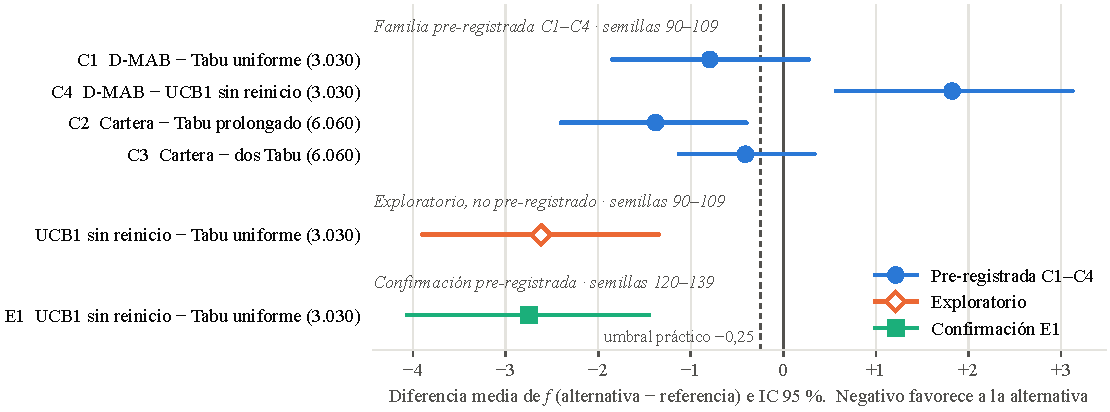
\includegraphics{figuras/forest_comparaciones}
 \caption{Diferencia media de $f$ e IC~95~\%; negativo favorece a la alternativa. Cada grupo es un análisis distinto.}
 \label{fig:forest}
\end{figure}

\subsection{La mejora de UCB1 cuesta cómputo y dispersión}
\label{subsec:costo}
Igual número de evaluaciones no significa igual cómputo. UCB1 repite más candidatos:
decodificó 10,1~\% más propuestas que Tabu uniforme y tardó 10,2~\% más (9,8~\%
en E1). D-MAB tardó 4,0~\% más.
% fuente: D (decoded_overhead, time_overhead)
UCB1 también fue más variable entre semillas, con DE de 9,36 frente a 8,72. En E1
se repitió el patrón: 9,89 frente a 8,90.
% fuente: D (sd)
La Figura~\ref{fig:distribucion} muestra que las distribuciones se superponen y que
la ventaja media de UCB1 se mantiene hasta el final.

En el piloto a igual tiempo, D-MAB fue peor que Tabu uniforme en tres de los cuatro
tamaños: $+0{,}21$, $-2{,}30$, $+2{,}70$ y $+6{,}00$. Son solo cinco semillas
por tamaño y el piloto no incluyó UCB1.
% fuente: R/entrega2_tiempo_110_114/summary.csv

\begin{figure}[!ht]
 \centering
 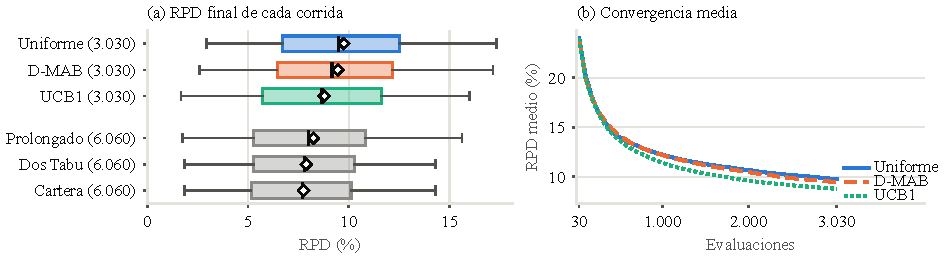
\includegraphics{figuras/distribucion_convergencia}
 \caption{Semillas 90--109. (a) RPD de 960 corridas por método: caja intercuartil, mediana, media (rombo) y percentiles 5--95. (b) RPD medio del mejor valor durante la búsqueda.}
 \label{fig:distribucion}
\end{figure}

\subsection{En el catálogo estándar los efectos no fueron consistentes}
\label{subsec:estandar}
Con la configuración vigente (semillas 40--59), los signos se invirtieron respecto
de la congestión. UCB1
menos uniforme dio $+1{,}182$; D-MAB menos uniforme, $+0{,}577$; y D-MAB menos
UCB1, $-0{,}605$.
% fuente: D (40-59)
Con la configuración anterior (semillas 20--39, $c=1$, $\lambda=0{,}35$), esas diferencias fueron
$-0{,}455$, $-0{,}513$ y $-0{,}058$.
% fuente: D (20-39)
En las semillas 60--79, D-MAB dio $+0{,}108$ frente a uniforme. La cartera dio
$-0{,}656$ frente al prolongado y $+0{,}134$ frente a dos Tabu.
% fuente: D (60-79)
Son descriptivos, con 12 instancias, y ninguno sustenta una superioridad.

\subsection{Discusión: bajo congestión ayuda UCB1, no el reinicio}
\label{subsec:discusion}
Los resultados responden la pregunta solo bajo escasez de cirujanos e igual número
de evaluaciones. Allí no identificamos una mejora concluyente de
D-MAB, mientras que UCB1 sí mejora, sobre todo desde 20 cirugías. La evidencia
señala al reinicio, con la configuración probada, como perjudicial en ese catálogo.
No demuestra que toda detección de cambios lo sea.

Una explicación plausible es que el detector confunde el agotamiento normal de la
búsqueda con un cambio entre operadores. Page--Hinkley detecta caídas de recompensa,
y las mejoras escasean al estancarse la búsqueda. D-MAB reinició una mediana de 24
veces por corrida, y cada reinicio borra sus estimaciones.
% fuente: R/entrega3_descriptivos/descriptivos.csv
La reparación no basta para explicarlo, porque afecta a todos. Alteró 46,6~\% de los
candidatos en uniforme, 44,0~\% en D-MAB y 40,1~\% en UCB1.
% fuente: R/entrega3_descriptivos/descriptivos.csv
Como no medimos si cambia el mejor operador, el mecanismo sigue siendo una hipótesis.

Este hallazgo concuerda con una parte de \textcite{dacosta2008}. En su escenario de
recompensas binarias, de alta varianza, el bandido sin reinicio superó a D-MAB.
Nuestra señal también es irregular: en el diagnóstico estándar, solo 3,9~\% de las
propuestas recibió recompensa positiva.
% fuente: R/entrega2_diagnostico_115_119/summary.csv
\textcite{dolatkhah2026} reinician con otra regla, una brecha entre operadores, por
lo que su resultado no valida este detector. \textcite{yin2026} miden brechas
frente a cotas; nuestro RPD, en cambio, no mide la distancia al óptimo.

E1 tampoco prueba que aprender sea la causa. UCB1 dedicó 39,1~\% de sus evaluaciones
al cambio de sala de anestesia, frente a 19,6~\% del uniforme.
% fuente: D (share_room_1)
Una mezcla fija con ese sesgo podría igualarlo. Además, confirmar con semillas
nuevas sobre las mismas instancias no mide generalización. Tampoco evaluamos
una cartera con UCB1.%
\label{res-fin}

% Cada cifra lleva su fuente en un comentario «% fuente: ruta».
% R = experiments/results. Las tablas y las figuras se generan con scripts.
% D = R/entrega3_revision/descriptivos.csv (descriptivo, no prerregistrado).
\section{Resultados y discusión}
\label{sec:resultados}\label{res-ini}
% Evita líneas viudas y huérfanas en esta sección y en la conclusión.
% \@clubpenalty es el valor que LaTeX restaura después de cada título.
\makeatletter\@clubpenalty=10000\makeatother
\clubpenalty=10000\widowpenalty=10000

\subsection{Tabu aporta la mayor parte de la mejora}
\label{subsec:absolutos}
El estudio completó los 960 pares sin fallos y su auditoría recalculó los 5.760
calendarios, todos factibles.
% fuente: R/entrega2_congestion_90_109/verification.json
El 51,8~\% de las soluciones de Tabu uniforme y D-MAB terminó con espera, entre
45,0~\% y 57,5~\% según el tamaño.
% fuente: R/entrega2_exploratorio/espera_por_tamano.csv
La Tabla~\ref{tab:descriptiva} muestra que Tabu uniforme ya mejora en 11,2~\% a la
mejor regla constructiva. UCB1 llega a 12,0~\%: cambiar la selección agrega menos de un
punto.
% fuente: D (improvement_over_best_rule)

\begin{table}[!ht]
 \centering
 \caption{Resultados en congestión (48 instancias, semillas 90--109; menor es mejor). RPD: respecto del mejor valor conocido, no del óptimo. Negrita: menor valor de cada bloque.}
 \label{tab:descriptiva}
 \scriptsize\setlength{\tabcolsep}{4pt}
 % Generado por experiments/scripts/tabla_descriptiva.py. No editar a mano.
% fuente: experiments/results/entrega3_revision/descriptivos.csv
\begin{tabular}{@{}lrrrrrrrrr@{}}
 \toprule
 & \multicolumn{5}{c}{Objetivo $f$ (unidades)} & \multicolumn{3}{c}{Componentes (min)} & \\
 \cmidrule(lr){2-6}\cmidrule(lr){7-9}
 Método & Mejor & Media & Peor & DE & RPD (\%) & $C_{\max}$ & $\sum W$ & $\max W$ & $t$ (s)\\
 \midrule
 FIFO & -- & 358,94 & -- & -- & 33,24 & 266,46 & 105,18 & 28,49 & --\\
 SPT & -- & 352,94 & -- & -- & 30,37 & 266,60 & 103,19 & 24,81 & --\\
 LPT & -- & 364,31 & -- & -- & 36,26 & 272,34 & 94,82 & 31,82 & --\\
 \midrule
 \multicolumn{10}{@{}l}{\emph{3.030 evaluaciones}}\\
 Uniforme & 280,31 & 297,20 & 312,80 & \textbf{8,72} & 9,75 & 287,56 & 9,31 & 3,55 & \textbf{6,17}\\
 D-MAB & 279,32 & 296,40 & 312,88 & 8,85 & 9,46 & 287,79 & 8,29 & 3,19 & 6,51\\
 UCB1 & \textbf{277,21} & \textbf{294,58} & \textbf{311,79} & 9,36 & \textbf{8,79} & \textbf{287,47} & \textbf{6,68} & \textbf{2,69} & 6,77\\
 \midrule
 \multicolumn{10}{@{}l}{\emph{6.060 evaluaciones}}\\
 Prolongado & 277,81 & 293,23 & 307,97 & 7,95 & 8,25 & 286,10 & \textbf{6,83} & \textbf{2,64} & \textbf{12,43}\\
 Dos Tabu & 277,87 & 292,26 & 305,89 & \textbf{7,29} & 7,89 & 284,74 & 7,16 & 2,81 & 12,59\\
 Cartera & \textbf{277,15} & \textbf{291,85} & \textbf{304,91} & \textbf{7,29} & \textbf{7,76} & \textbf{284,45} & 6,99 & 2,78 & 12,87\\
 \bottomrule
\end{tabular}

\end{table}

\subsection{La evidencia sobre D-MAB frente a Tabu uniforme no es concluyente}
\label{subsec:c1}
En C1 (Tabla~\ref{tab:comparaciones}), la diferencia media fue $-0{,}793$, con
IC~95~\% [$-1{,}850$; $+0{,}279$] y $p$ de Holm 0,041.
% fuente: R/entrega2_congestion_90_109/comparisons.csv (C1)
Wilcoxon rechaza la igualdad, pero el intervalo incluye el cero. Por tanto, la regla
prerregistrada no respalda la hipótesis primaria. El desacuerdo se relaciona con el
bootstrap: su error estándar es 1,62 veces el de las medias por instancia.
% fuente: D (bootstrap_se_ratio, C1)
Aunque es conservador, se fijó antes y no lo cambiamos.

El intervalo incluye beneficios y perjuicios mayores que el umbral de 0,25. Además,
la DE de las diferencias fue 13,21 y no la supuesta de 7,03. Así, la potencia para
detectar 0,65 cayó a 0,32, y el resultado no prueba equivalencia.
% fuente: R/entrega2_exploratorio/potencia_realizada.csv
La espera total bajó con D-MAB de 9,31 a 8,29 minutos. El \emph{makespan}, en
cambio, subió levemente, de 287,56 a 287,79.
% fuente: R/entrega2_congestion_90_109/descriptive.csv

\begin{table}[!ht]
 \centering
 \caption{Diferencias de $f$, en unidades del objetivo (semillas 90--109, 960 pares); negativo favorece a la alternativa. Negrita: cumple los tres criterios de la regla, que solo era vinculante para C1. Las columnas por tamaño son descriptivas, con 12 instancias cada una.}
 \label{tab:comparaciones}
 \scriptsize\setlength{\tabcolsep}{4pt}
 % Generado por experiments/scripts/tabla_resultados.py. No editar a mano.
% fuente: experiments/results/entrega2_congestion_90_109/comparisons.csv
% fuente de las columnas por tamaño: experiments/results/entrega3_revision/descriptivos.csv
\begin{tabular}{@{}llrcrrrrr@{}}
 \toprule
 & & & & & \multicolumn{4}{c}{Media por n.º de cirugías}\\
 \cmidrule(l){6-9}
 Id & Alternativa $-$ referencia & Media & IC 95~\% & $p$ Holm & 15 & 20 & 25 & 30\\
 \midrule
 \multicolumn{9}{@{}l}{\emph{3.030 evaluaciones por método}}\\
 C1 & D-MAB $-$ uniforme & $-0{,}793$ & [$-1{,}850$; $+0{,}279$] & $0{,}041$ & $-0{,}51$ & $-0{,}44$ & $-0{,}12$ & $-2{,}10$\\
 C4 & D-MAB $-$ UCB1 & $\mathbf{+1{,}824}$ & [$+0{,}566$; $+3{,}124$] & $0{,}005$ & $-0{,}98$ & $+1{,}40$ & $+4{,}95$ & $+1{,}93$\\
 \midrule
 \multicolumn{9}{@{}l}{\emph{6.060 evaluaciones por método}}\\
 C2 & Cartera $-$ prolongado & $\mathbf{-1{,}380}$ & [$-2{,}405$; $-0{,}398$] & $0{,}008$ & $+0{,}70$ & $+0{,}19$ & $-1{,}98$ & $-4{,}43$\\
 C3 & Cartera $-$ dos Tabu & $-0{,}409$ & [$-1{,}126$; $+0{,}338$] & $0{,}057$ & $-0{,}12$ & $-0{,}31$ & $+0{,}37$ & $-1{,}58$\\
 \bottomrule
\end{tabular}

\end{table}

\subsection{La cartera gana al prolongado, pero no a repetir la búsqueda}
\label{subsec:cartera}
La cartera superó al Tabu prolongado (C2), pero no se distinguió de dos Tabu
independientes (C3). Por tanto, no atribuimos su ganancia al aprendizaje. La
explicación más simple es el estancamiento. En 546 de las 960 corridas (56,9~\%),
el Tabu prolongado no mejoró después de la evaluación 3.030.
% fuente: R/entrega3_descriptivos/descriptivos.csv
La ventaja aparece con 25 y 30 cirugías; con 15 y 20, la cartera es peor en media.
Además, el error tipo~I simulado de C2 fue 0,082.
% fuente: R/entrega2_potencia/simulacion.csv

\subsection{UCB1 supera a D-MAB y a Tabu uniforme, según el tamaño}
\label{subsec:reinicio}
En C4, quitar el reinicio mejoró el resultado: con 25 cirugías, UCB1 venció a D-MAB
en las 12 instancias.
% fuente: D (instances_better_25, C4)
Con 15, en cambio, D-MAB fue mejor en media. El contraste exploratorio entre UCB1
y Tabu uniforme había dado $-2{,}617$.
% fuente: R/entrega2_exploratorio/contrastes.csv
Por eso, lo confirmamos con un protocolo propio y semillas nuevas. En E1, la
diferencia fue $-2{,}749$, con IC [$-4{,}069$; $-1{,}453$] y $p$ menor que 0,001
(Figura~\ref{fig:forest}).
% fuente: R/entrega3_confirmacion_ucb1/comparisons.csv (E1)

E1 cumple la regla y mejora en 38 de 48 instancias, pero equivale a solo 0,92~\%
de $f$. Además, depende del tamaño. Con 15, 20, 25 y 30 cirugías dio $+0{,}12$,
$-2{,}96$, $-3{,}91$ y $-4{,}25$: con 15 no hay ventaja.
% fuente: D (instances_better, relative_difference y difference_<tamaño>, E1)

\begin{figure}[!ht]
 \centering
 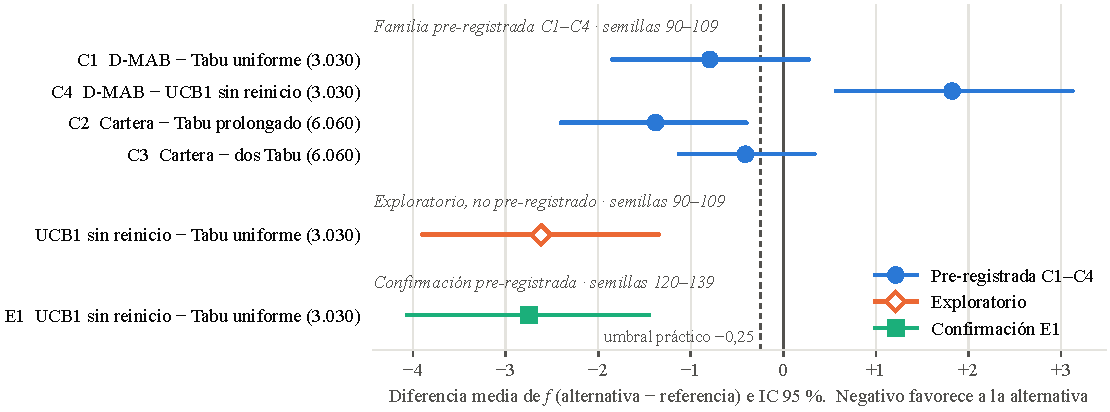
\includegraphics{figuras/forest_comparaciones}
 \caption{Diferencia media de $f$ e IC~95~\%; negativo favorece a la alternativa. Cada grupo es un análisis distinto.}
 \label{fig:forest}
\end{figure}

\subsection{La mejora de UCB1 cuesta cómputo y dispersión}
\label{subsec:costo}
Igual número de evaluaciones no significa igual cómputo. UCB1 repite más candidatos:
decodificó 10,1~\% más propuestas que Tabu uniforme y tardó 10,2~\% más (9,8~\%
en E1). D-MAB tardó 4,0~\% más.
% fuente: D (decoded_overhead, time_overhead)
UCB1 también fue más variable entre semillas, con DE de 9,36 frente a 8,72. En E1
se repitió el patrón: 9,89 frente a 8,90.
% fuente: D (sd)
La Figura~\ref{fig:distribucion} muestra que las distribuciones se superponen y que
la ventaja media de UCB1 se mantiene hasta el final.

En el piloto a igual tiempo, D-MAB fue peor que Tabu uniforme en tres de los cuatro
tamaños: $+0{,}21$, $-2{,}30$, $+2{,}70$ y $+6{,}00$. Son solo cinco semillas
por tamaño y el piloto no incluyó UCB1.
% fuente: R/entrega2_tiempo_110_114/summary.csv

\begin{figure}[!ht]
 \centering
 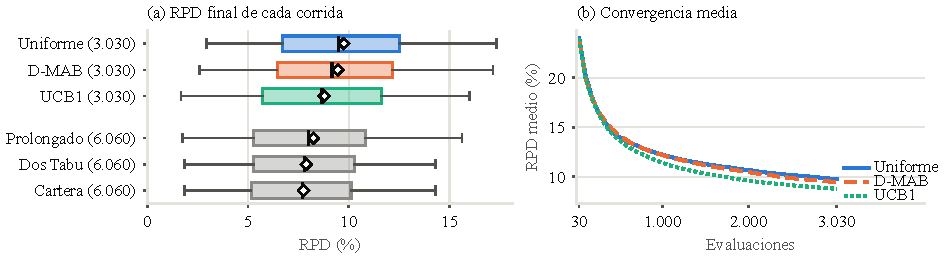
\includegraphics{figuras/distribucion_convergencia}
 \caption{Semillas 90--109. (a) RPD de 960 corridas por método: caja intercuartil, mediana, media (rombo) y percentiles 5--95. (b) RPD medio del mejor valor durante la búsqueda.}
 \label{fig:distribucion}
\end{figure}

\subsection{En el catálogo estándar los efectos no fueron consistentes}
\label{subsec:estandar}
Con la configuración vigente (semillas 40--59), los signos se invirtieron respecto
de la congestión. UCB1
menos uniforme dio $+1{,}182$; D-MAB menos uniforme, $+0{,}577$; y D-MAB menos
UCB1, $-0{,}605$.
% fuente: D (40-59)
Con la configuración anterior (semillas 20--39, $c=1$, $\lambda=0{,}35$), esas diferencias fueron
$-0{,}455$, $-0{,}513$ y $-0{,}058$.
% fuente: D (20-39)
En las semillas 60--79, D-MAB dio $+0{,}108$ frente a uniforme. La cartera dio
$-0{,}656$ frente al prolongado y $+0{,}134$ frente a dos Tabu.
% fuente: D (60-79)
Son descriptivos, con 12 instancias, y ninguno sustenta una superioridad.

\subsection{Discusión: bajo congestión ayuda UCB1, no el reinicio}
\label{subsec:discusion}
Los resultados responden la pregunta solo bajo escasez de cirujanos e igual número
de evaluaciones. Allí no identificamos una mejora concluyente de
D-MAB, mientras que UCB1 sí mejora, sobre todo desde 20 cirugías. La evidencia
señala al reinicio, con la configuración probada, como perjudicial en ese catálogo.
No demuestra que toda detección de cambios lo sea.

Una explicación plausible es que el detector confunde el agotamiento normal de la
búsqueda con un cambio entre operadores. Page--Hinkley detecta caídas de recompensa,
y las mejoras escasean al estancarse la búsqueda. D-MAB reinició una mediana de 24
veces por corrida, y cada reinicio borra sus estimaciones.
% fuente: R/entrega3_descriptivos/descriptivos.csv
La reparación no basta para explicarlo, porque afecta a todos. Alteró 46,6~\% de los
candidatos en uniforme, 44,0~\% en D-MAB y 40,1~\% en UCB1.
% fuente: R/entrega3_descriptivos/descriptivos.csv
Como no medimos si cambia el mejor operador, el mecanismo sigue siendo una hipótesis.

Este hallazgo concuerda con una parte de \textcite{dacosta2008}. En su escenario de
recompensas binarias, de alta varianza, el bandido sin reinicio superó a D-MAB.
Nuestra señal también es irregular: en el diagnóstico estándar, solo 3,9~\% de las
propuestas recibió recompensa positiva.
% fuente: R/entrega2_diagnostico_115_119/summary.csv
\textcite{dolatkhah2026} reinician con otra regla, una brecha entre operadores, por
lo que su resultado no valida este detector. \textcite{yin2026} miden brechas
frente a cotas; nuestro RPD, en cambio, no mide la distancia al óptimo.

E1 tampoco prueba que aprender sea la causa. UCB1 dedicó 39,1~\% de sus evaluaciones
al cambio de sala de anestesia, frente a 19,6~\% del uniforme.
% fuente: D (share_room_1)
Una mezcla fija con ese sesgo podría igualarlo. Además, confirmar con semillas
nuevas sobre las mismas instancias no mide generalización. Tampoco evaluamos
una cartera con UCB1.%
\label{res-fin}

% Cada cifra lleva su fuente en un comentario «% fuente: ruta».
% R = experiments/results. Las tablas y las figuras se generan con scripts.
% D = R/entrega3_revision/descriptivos.csv (descriptivo, no prerregistrado).
\section{Resultados y discusión}
\label{sec:resultados}\label{res-ini}
% Evita líneas viudas y huérfanas en esta sección y en la conclusión.
% \@clubpenalty es el valor que LaTeX restaura después de cada título.
\makeatletter\@clubpenalty=10000\makeatother
\clubpenalty=10000\widowpenalty=10000

\subsection{Tabu aporta la mayor parte de la mejora}
\label{subsec:absolutos}
El estudio completó los 960 pares sin fallos y su auditoría recalculó los 5.760
calendarios, todos factibles.
% fuente: R/entrega2_congestion_90_109/verification.json
El 51,8~\% de las soluciones de Tabu uniforme y D-MAB terminó con espera, entre
45,0~\% y 57,5~\% según el tamaño.
% fuente: R/entrega2_exploratorio/espera_por_tamano.csv
La Tabla~\ref{tab:descriptiva} muestra que Tabu uniforme ya mejora en 11,2~\% a la
mejor regla constructiva. UCB1 llega a 12,0~\%: cambiar la selección agrega menos de un
punto.
% fuente: D (improvement_over_best_rule)

\begin{table}[!ht]
 \centering
 \caption{Resultados en congestión (48 instancias, semillas 90--109; menor es mejor). RPD: respecto del mejor valor conocido, no del óptimo. Negrita: menor valor de cada bloque.}
 \label{tab:descriptiva}
 \scriptsize\setlength{\tabcolsep}{4pt}
 % Generado por experiments/scripts/tabla_descriptiva.py. No editar a mano.
% fuente: experiments/results/entrega3_revision/descriptivos.csv
\begin{tabular}{@{}lrrrrrrrrr@{}}
 \toprule
 & \multicolumn{5}{c}{Objetivo $f$ (unidades)} & \multicolumn{3}{c}{Componentes (min)} & \\
 \cmidrule(lr){2-6}\cmidrule(lr){7-9}
 Método & Mejor & Media & Peor & DE & RPD (\%) & $C_{\max}$ & $\sum W$ & $\max W$ & $t$ (s)\\
 \midrule
 FIFO & -- & 358,94 & -- & -- & 33,24 & 266,46 & 105,18 & 28,49 & --\\
 SPT & -- & 352,94 & -- & -- & 30,37 & 266,60 & 103,19 & 24,81 & --\\
 LPT & -- & 364,31 & -- & -- & 36,26 & 272,34 & 94,82 & 31,82 & --\\
 \midrule
 \multicolumn{10}{@{}l}{\emph{3.030 evaluaciones}}\\
 Uniforme & 280,31 & 297,20 & 312,80 & \textbf{8,72} & 9,75 & 287,56 & 9,31 & 3,55 & \textbf{6,17}\\
 D-MAB & 279,32 & 296,40 & 312,88 & 8,85 & 9,46 & 287,79 & 8,29 & 3,19 & 6,51\\
 UCB1 & \textbf{277,21} & \textbf{294,58} & \textbf{311,79} & 9,36 & \textbf{8,79} & \textbf{287,47} & \textbf{6,68} & \textbf{2,69} & 6,77\\
 \midrule
 \multicolumn{10}{@{}l}{\emph{6.060 evaluaciones}}\\
 Prolongado & 277,81 & 293,23 & 307,97 & 7,95 & 8,25 & 286,10 & \textbf{6,83} & \textbf{2,64} & \textbf{12,43}\\
 Dos Tabu & 277,87 & 292,26 & 305,89 & \textbf{7,29} & 7,89 & 284,74 & 7,16 & 2,81 & 12,59\\
 Cartera & \textbf{277,15} & \textbf{291,85} & \textbf{304,91} & \textbf{7,29} & \textbf{7,76} & \textbf{284,45} & 6,99 & 2,78 & 12,87\\
 \bottomrule
\end{tabular}

\end{table}

\subsection{La evidencia sobre D-MAB frente a Tabu uniforme no es concluyente}
\label{subsec:c1}
En C1 (Tabla~\ref{tab:comparaciones}), la diferencia media fue $-0{,}793$, con
IC~95~\% [$-1{,}850$; $+0{,}279$] y $p$ de Holm 0,041.
% fuente: R/entrega2_congestion_90_109/comparisons.csv (C1)
Wilcoxon rechaza la igualdad, pero el intervalo incluye el cero. Por tanto, la regla
prerregistrada no respalda la hipótesis primaria. El desacuerdo se relaciona con el
bootstrap: su error estándar es 1,62 veces el de las medias por instancia.
% fuente: D (bootstrap_se_ratio, C1)
Aunque es conservador, se fijó antes y no lo cambiamos.

El intervalo incluye beneficios y perjuicios mayores que el umbral de 0,25. Además,
la DE de las diferencias fue 13,21 y no la supuesta de 7,03. Así, la potencia para
detectar 0,65 cayó a 0,32, y el resultado no prueba equivalencia.
% fuente: R/entrega2_exploratorio/potencia_realizada.csv
La espera total bajó con D-MAB de 9,31 a 8,29 minutos. El \emph{makespan}, en
cambio, subió levemente, de 287,56 a 287,79.
% fuente: R/entrega2_congestion_90_109/descriptive.csv

\begin{table}[!ht]
 \centering
 \caption{Diferencias de $f$, en unidades del objetivo (semillas 90--109, 960 pares); negativo favorece a la alternativa. Negrita: cumple los tres criterios de la regla, que solo era vinculante para C1. Las columnas por tamaño son descriptivas, con 12 instancias cada una.}
 \label{tab:comparaciones}
 \scriptsize\setlength{\tabcolsep}{4pt}
 % Generado por experiments/scripts/tabla_resultados.py. No editar a mano.
% fuente: experiments/results/entrega2_congestion_90_109/comparisons.csv
% fuente de las columnas por tamaño: experiments/results/entrega3_revision/descriptivos.csv
\begin{tabular}{@{}llrcrrrrr@{}}
 \toprule
 & & & & & \multicolumn{4}{c}{Media por n.º de cirugías}\\
 \cmidrule(l){6-9}
 Id & Alternativa $-$ referencia & Media & IC 95~\% & $p$ Holm & 15 & 20 & 25 & 30\\
 \midrule
 \multicolumn{9}{@{}l}{\emph{3.030 evaluaciones por método}}\\
 C1 & D-MAB $-$ uniforme & $-0{,}793$ & [$-1{,}850$; $+0{,}279$] & $0{,}041$ & $-0{,}51$ & $-0{,}44$ & $-0{,}12$ & $-2{,}10$\\
 C4 & D-MAB $-$ UCB1 & $\mathbf{+1{,}824}$ & [$+0{,}566$; $+3{,}124$] & $0{,}005$ & $-0{,}98$ & $+1{,}40$ & $+4{,}95$ & $+1{,}93$\\
 \midrule
 \multicolumn{9}{@{}l}{\emph{6.060 evaluaciones por método}}\\
 C2 & Cartera $-$ prolongado & $\mathbf{-1{,}380}$ & [$-2{,}405$; $-0{,}398$] & $0{,}008$ & $+0{,}70$ & $+0{,}19$ & $-1{,}98$ & $-4{,}43$\\
 C3 & Cartera $-$ dos Tabu & $-0{,}409$ & [$-1{,}126$; $+0{,}338$] & $0{,}057$ & $-0{,}12$ & $-0{,}31$ & $+0{,}37$ & $-1{,}58$\\
 \bottomrule
\end{tabular}

\end{table}

\subsection{La cartera gana al prolongado, pero no a repetir la búsqueda}
\label{subsec:cartera}
La cartera superó al Tabu prolongado (C2), pero no se distinguió de dos Tabu
independientes (C3). Por tanto, no atribuimos su ganancia al aprendizaje. La
explicación más simple es el estancamiento. En 546 de las 960 corridas (56,9~\%),
el Tabu prolongado no mejoró después de la evaluación 3.030.
% fuente: R/entrega3_descriptivos/descriptivos.csv
La ventaja aparece con 25 y 30 cirugías; con 15 y 20, la cartera es peor en media.
Además, el error tipo~I simulado de C2 fue 0,082.
% fuente: R/entrega2_potencia/simulacion.csv

\subsection{UCB1 supera a D-MAB y a Tabu uniforme, según el tamaño}
\label{subsec:reinicio}
En C4, quitar el reinicio mejoró el resultado: con 25 cirugías, UCB1 venció a D-MAB
en las 12 instancias.
% fuente: D (instances_better_25, C4)
Con 15, en cambio, D-MAB fue mejor en media. El contraste exploratorio entre UCB1
y Tabu uniforme había dado $-2{,}617$.
% fuente: R/entrega2_exploratorio/contrastes.csv
Por eso, lo confirmamos con un protocolo propio y semillas nuevas. En E1, la
diferencia fue $-2{,}749$, con IC [$-4{,}069$; $-1{,}453$] y $p$ menor que 0,001
(Figura~\ref{fig:forest}).
% fuente: R/entrega3_confirmacion_ucb1/comparisons.csv (E1)

E1 cumple la regla y mejora en 38 de 48 instancias, pero equivale a solo 0,92~\%
de $f$. Además, depende del tamaño. Con 15, 20, 25 y 30 cirugías dio $+0{,}12$,
$-2{,}96$, $-3{,}91$ y $-4{,}25$: con 15 no hay ventaja.
% fuente: D (instances_better, relative_difference y difference_<tamaño>, E1)

\begin{figure}[!ht]
 \centering
 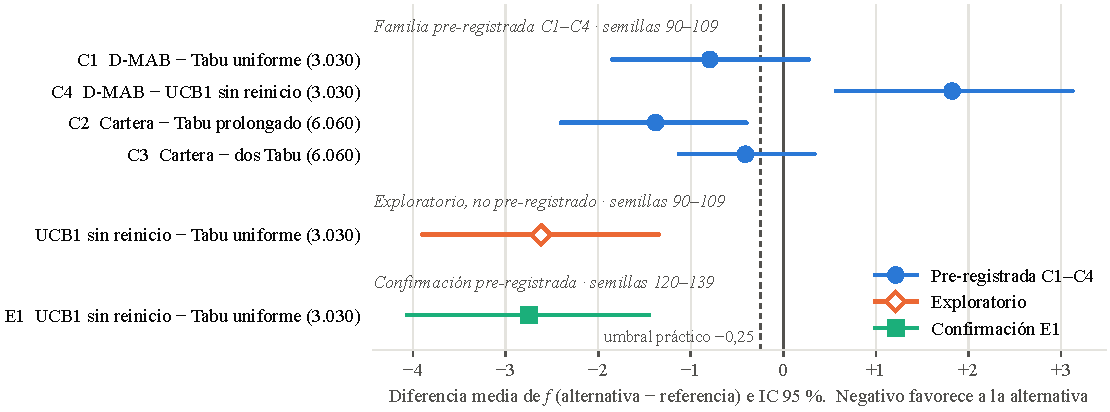
\includegraphics{figuras/forest_comparaciones}
 \caption{Diferencia media de $f$ e IC~95~\%; negativo favorece a la alternativa. Cada grupo es un análisis distinto.}
 \label{fig:forest}
\end{figure}

\subsection{La mejora de UCB1 cuesta cómputo y dispersión}
\label{subsec:costo}
Igual número de evaluaciones no significa igual cómputo. UCB1 repite más candidatos:
decodificó 10,1~\% más propuestas que Tabu uniforme y tardó 10,2~\% más (9,8~\%
en E1). D-MAB tardó 4,0~\% más.
% fuente: D (decoded_overhead, time_overhead)
UCB1 también fue más variable entre semillas, con DE de 9,36 frente a 8,72. En E1
se repitió el patrón: 9,89 frente a 8,90.
% fuente: D (sd)
La Figura~\ref{fig:distribucion} muestra que las distribuciones se superponen y que
la ventaja media de UCB1 se mantiene hasta el final.

En el piloto a igual tiempo, D-MAB fue peor que Tabu uniforme en tres de los cuatro
tamaños: $+0{,}21$, $-2{,}30$, $+2{,}70$ y $+6{,}00$. Son solo cinco semillas
por tamaño y el piloto no incluyó UCB1.
% fuente: R/entrega2_tiempo_110_114/summary.csv

\begin{figure}[!ht]
 \centering
 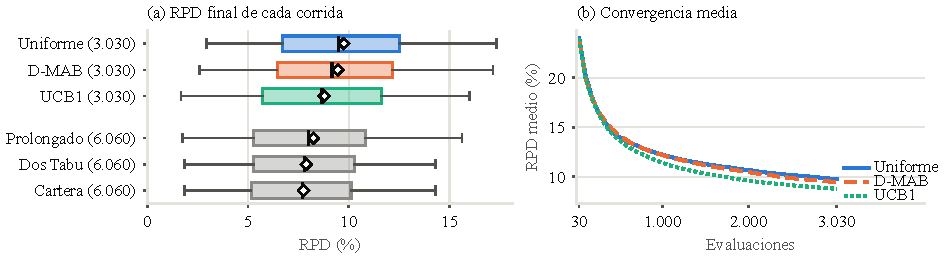
\includegraphics{figuras/distribucion_convergencia}
 \caption{Semillas 90--109. (a) RPD de 960 corridas por método: caja intercuartil, mediana, media (rombo) y percentiles 5--95. (b) RPD medio del mejor valor durante la búsqueda.}
 \label{fig:distribucion}
\end{figure}

\subsection{En el catálogo estándar los efectos no fueron consistentes}
\label{subsec:estandar}
Con la configuración vigente (semillas 40--59), los signos se invirtieron respecto
de la congestión. UCB1
menos uniforme dio $+1{,}182$; D-MAB menos uniforme, $+0{,}577$; y D-MAB menos
UCB1, $-0{,}605$.
% fuente: D (40-59)
Con la configuración anterior (semillas 20--39, $c=1$, $\lambda=0{,}35$), esas diferencias fueron
$-0{,}455$, $-0{,}513$ y $-0{,}058$.
% fuente: D (20-39)
En las semillas 60--79, D-MAB dio $+0{,}108$ frente a uniforme. La cartera dio
$-0{,}656$ frente al prolongado y $+0{,}134$ frente a dos Tabu.
% fuente: D (60-79)
Son descriptivos, con 12 instancias, y ninguno sustenta una superioridad.

\subsection{Discusión: bajo congestión ayuda UCB1, no el reinicio}
\label{subsec:discusion}
Los resultados responden la pregunta solo bajo escasez de cirujanos e igual número
de evaluaciones. Allí no identificamos una mejora concluyente de
D-MAB, mientras que UCB1 sí mejora, sobre todo desde 20 cirugías. La evidencia
señala al reinicio, con la configuración probada, como perjudicial en ese catálogo.
No demuestra que toda detección de cambios lo sea.

Una explicación plausible es que el detector confunde el agotamiento normal de la
búsqueda con un cambio entre operadores. Page--Hinkley detecta caídas de recompensa,
y las mejoras escasean al estancarse la búsqueda. D-MAB reinició una mediana de 24
veces por corrida, y cada reinicio borra sus estimaciones.
% fuente: R/entrega3_descriptivos/descriptivos.csv
La reparación no basta para explicarlo, porque afecta a todos. Alteró 46,6~\% de los
candidatos en uniforme, 44,0~\% en D-MAB y 40,1~\% en UCB1.
% fuente: R/entrega3_descriptivos/descriptivos.csv
Como no medimos si cambia el mejor operador, el mecanismo sigue siendo una hipótesis.

Este hallazgo concuerda con una parte de \textcite{dacosta2008}. En su escenario de
recompensas binarias, de alta varianza, el bandido sin reinicio superó a D-MAB.
Nuestra señal también es irregular: en el diagnóstico estándar, solo 3,9~\% de las
propuestas recibió recompensa positiva.
% fuente: R/entrega2_diagnostico_115_119/summary.csv
\textcite{dolatkhah2026} reinician con otra regla, una brecha entre operadores, por
lo que su resultado no valida este detector. \textcite{yin2026} miden brechas
frente a cotas; nuestro RPD, en cambio, no mide la distancia al óptimo.

E1 tampoco prueba que aprender sea la causa. UCB1 dedicó 39,1~\% de sus evaluaciones
al cambio de sala de anestesia, frente a 19,6~\% del uniforme.
% fuente: D (share_room_1)
Una mezcla fija con ese sesgo podría igualarlo. Además, confirmar con semillas
nuevas sobre las mismas instancias no mide generalización. Tampoco evaluamos
una cartera con UCB1.%
\label{res-fin}
